\documentclass[1p]{elsarticle_modified}
%\bibliographystyle{elsarticle-num}

%\usepackage[colorlinks]{hyperref}
%\usepackage{abbrmath_seonhwa} %\Abb, \Ascr, \Acal ,\Abf, \Afrak
\usepackage{amsfonts}
\usepackage{amssymb}
\usepackage{amsmath}
\usepackage{amsthm}
\usepackage{scalefnt}
\usepackage{amsbsy}
\usepackage{kotex}
\usepackage{caption}
\usepackage{subfig}
\usepackage{color}
\usepackage{graphicx}
\usepackage{xcolor} %% white, black, red, green, blue, cyan, magenta, yellow
\usepackage{float}
\usepackage{setspace}
\usepackage{hyperref}

\usepackage{tikz}
\usetikzlibrary{arrows}

\usepackage{multirow}
\usepackage{array} % fixed length table
\usepackage{hhline}

%%%%%%%%%%%%%%%%%%%%%
\makeatletter
\renewcommand*\env@matrix[1][\arraystretch]{%
	\edef\arraystretch{#1}%
	\hskip -\arraycolsep
	\let\@ifnextchar\new@ifnextchar
	\array{*\c@MaxMatrixCols c}}
\makeatother %https://tex.stackexchange.com/questions/14071/how-can-i-increase-the-line-spacing-in-a-matrix
%%%%%%%%%%%%%%%

\usepackage[normalem]{ulem}

\newcommand{\msout}[1]{\ifmmode\text{\sout{\ensuremath{#1}}}\else\sout{#1}\fi}
%SOURCE: \msout is \stkout macro in https://tex.stackexchange.com/questions/20609/strikeout-in-math-mode

\newcommand{\cancel}[1]{
	\ifmmode
	{\color{red}\msout{#1}}
	\else
	{\color{red}\sout{#1}}
	\fi
}

\newcommand{\add}[1]{
	{\color{blue}\uwave{#1}}
}

\newcommand{\replace}[2]{
	\ifmmode
	{\color{red}\msout{#1}}{\color{blue}\uwave{#2}}
	\else
	{\color{red}\sout{#1}}{\color{blue}\uwave{#2}}
	\fi
}

\newcommand{\Sol}{\mathcal{S}} %segment
\newcommand{\D}{D} %diagram
\newcommand{\A}{\mathcal{A}} %arc


%%%%%%%%%%%%%%%%%%%%%%%%%%%%%5 test

\def\sl{\operatorname{\textup{SL}}(2,\Cbb)}
\def\psl{\operatorname{\textup{PSL}}(2,\Cbb)}
\def\quan{\mkern 1mu \triangleright \mkern 1mu}

\theoremstyle{definition}
\newtheorem{thm}{Theorem}[section]
\newtheorem{prop}[thm]{Proposition}
\newtheorem{lem}[thm]{Lemma}
\newtheorem{ques}[thm]{Question}
\newtheorem{cor}[thm]{Corollary}
\newtheorem{defn}[thm]{Definition}
\newtheorem{exam}[thm]{Example}
\newtheorem{rmk}[thm]{Remark}
\newtheorem{alg}[thm]{Algorithm}

\newcommand{\I}{\sqrt{-1}}
\begin{document}

%\begin{frontmatter}
%
%\title{Boundary parabolic representations of knots up to 8 crossings}
%
%%% Group authors per affiliation:
%\author{Yunhi Cho} 
%\address{Department of Mathematics, University of Seoul, Seoul, Korea}
%\ead{yhcho@uos.ac.kr}
%
%
%\author{Seonhwa Kim} %\fnref{s_kim}}
%\address{Center for Geometry and Physics, Institute for Basic Science, Pohang, 37673, Korea}
%\ead{ryeona17@ibs.re.kr}
%
%\author{Hyuk Kim}
%\address{Department of Mathematical Sciences, Seoul National University, Seoul 08826, Korea}
%\ead{hyukkim@snu.ac.kr}
%
%\author{Seokbeom Yoon}
%\address{Department of Mathematical Sciences, Seoul National University, Seoul, 08826,  Korea}
%\ead{sbyoon15@snu.ac.kr}
%
%\begin{abstract}
%We find all boundary parabolic representation of knots up to 8 crossings.
%
%\end{abstract}
%\begin{keyword}
%    \MSC[2010] 57M25 
%\end{keyword}
%
%\end{frontmatter}

%\linenumbers
%\tableofcontents
%
\newcommand\colored[1]{\textcolor{white}{\rule[-0.35ex]{0.8em}{1.4ex}}\kern-0.8em\color{red} #1}%
%\newcommand\colored[1]{\textcolor{white}{ #1}\kern-2.17ex	\textcolor{white}{ #1}\kern-1.81ex	\textcolor{white}{ #1}\kern-2.15ex\color{red}#1	}

{\Large $\underline{11n_{118}~(K11n_{118})}$}

\setlength{\tabcolsep}{10pt}
\renewcommand{\arraystretch}{1.6}
\vspace{1cm}\begin{tabular}{m{100pt}>{\centering\arraybackslash}m{274pt}}
\multirow{5}{120pt}{
	\centering
	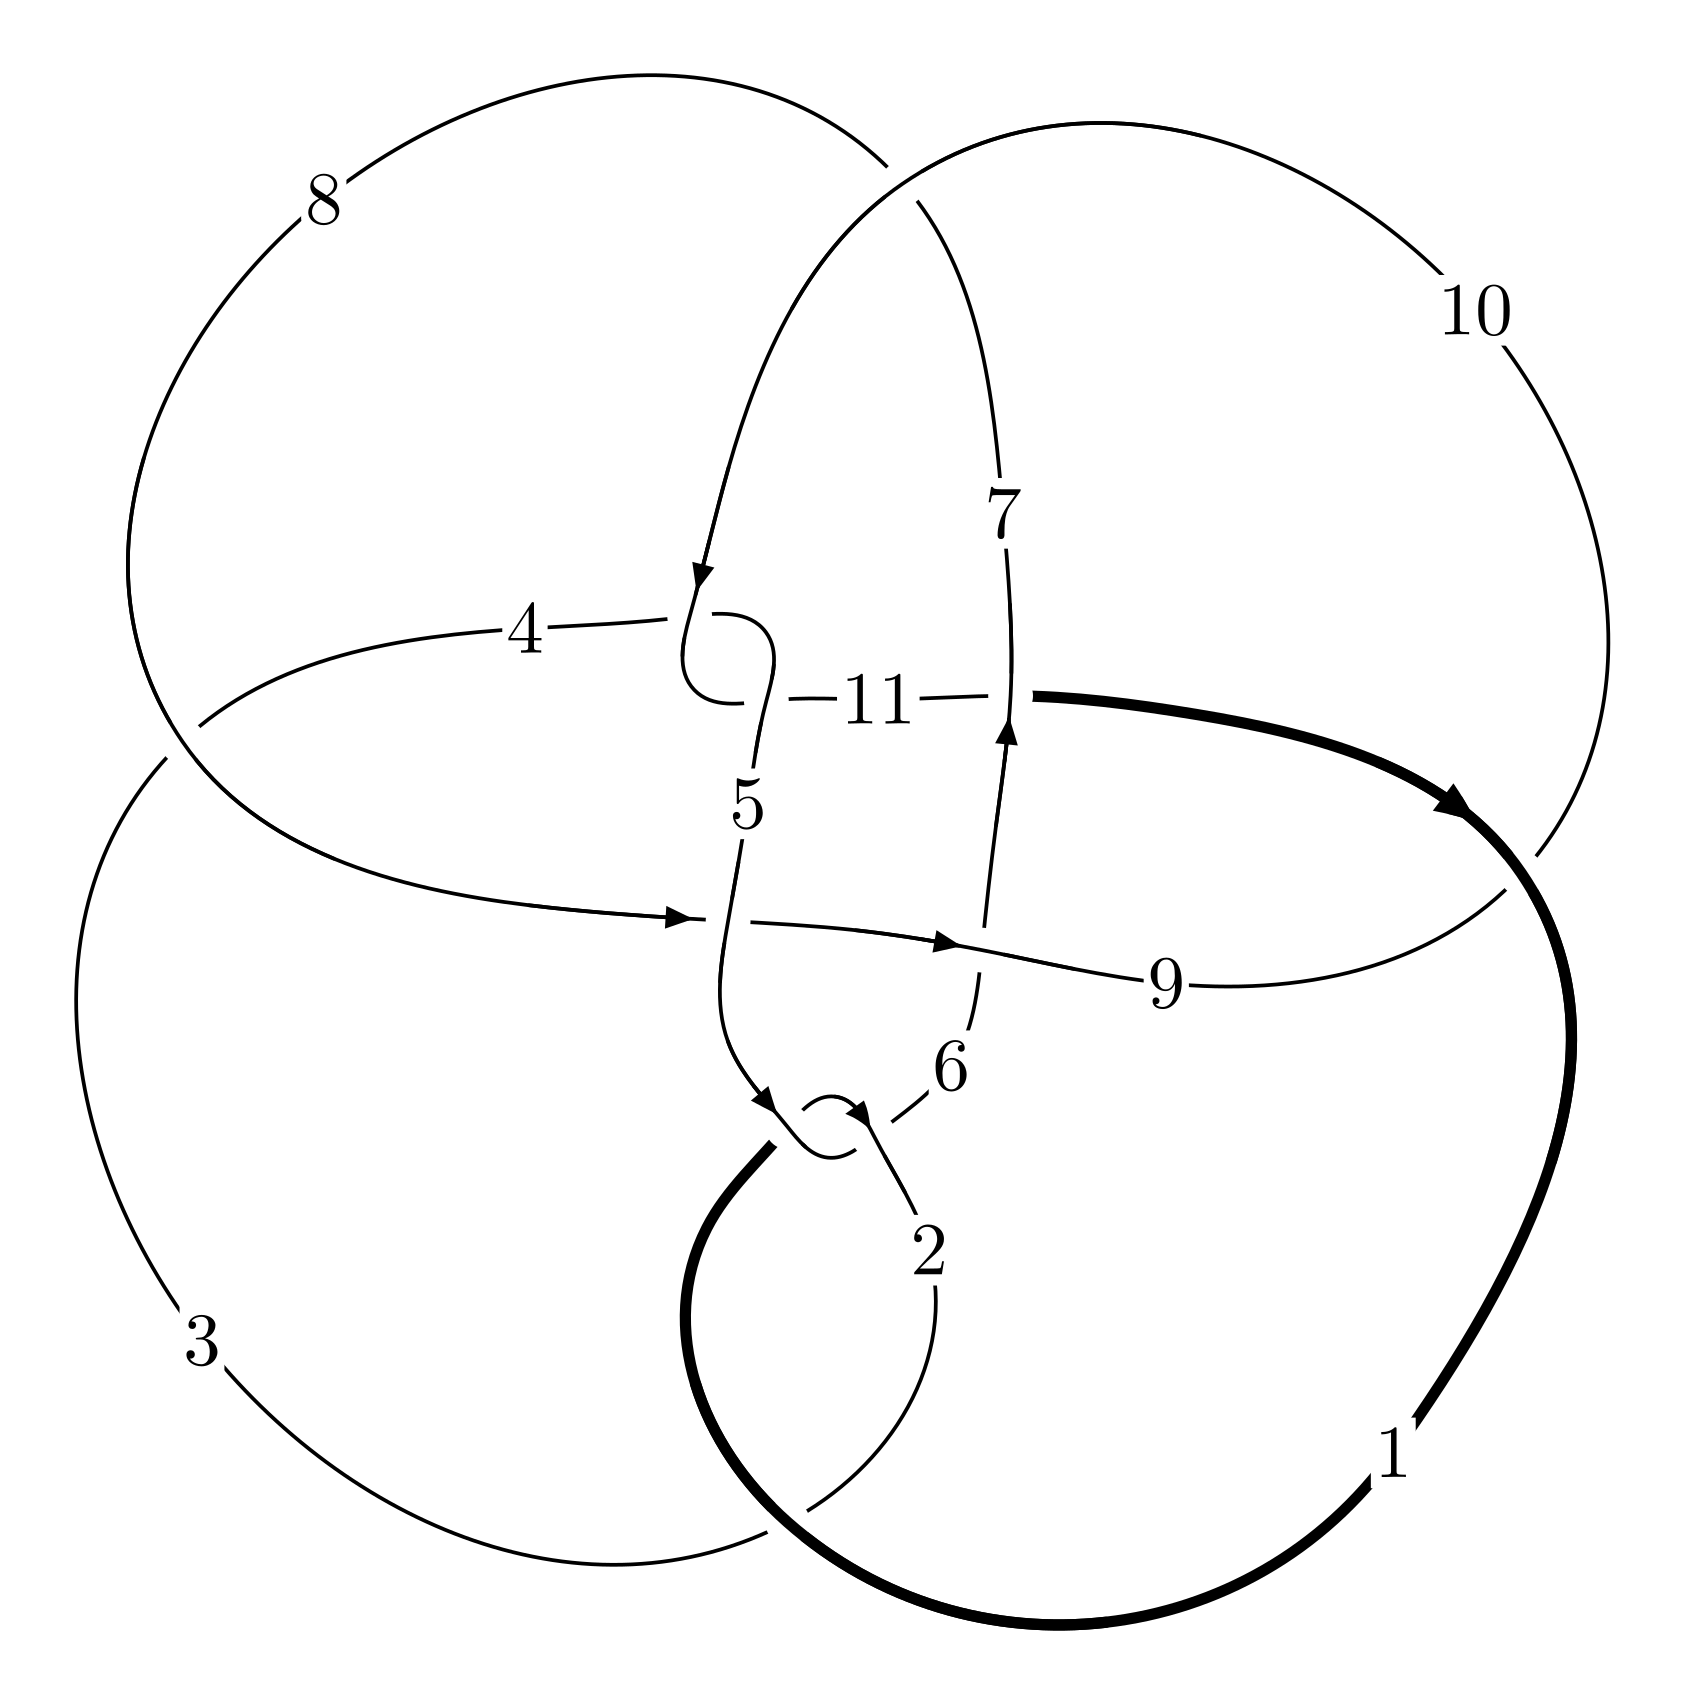
\includegraphics[width=112pt]{../../../GIT/diagram.site/Diagrams/png/734_11n_118.png}\\
\ \ \ A knot diagram\footnotemark}&
\allowdisplaybreaks
\textbf{Linearized knot diagam} \\
\cline{2-2}
 &
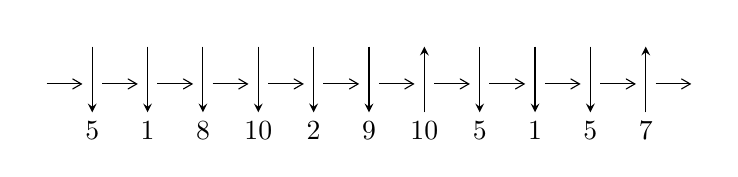
\begin{tikzpicture}[x=20pt, y=17pt]
	% nodes
	\node (C0) at (0, 0) {};
	\node (C1) at (1, 0) {};
	\node (C1U) at (1, +1) {};
	\node (C1D) at (1, -1) {5};

	\node (C2) at (2, 0) {};
	\node (C2U) at (2, +1) {};
	\node (C2D) at (2, -1) {1};

	\node (C3) at (3, 0) {};
	\node (C3U) at (3, +1) {};
	\node (C3D) at (3, -1) {8};

	\node (C4) at (4, 0) {};
	\node (C4U) at (4, +1) {};
	\node (C4D) at (4, -1) {10};

	\node (C5) at (5, 0) {};
	\node (C5U) at (5, +1) {};
	\node (C5D) at (5, -1) {2};

	\node (C6) at (6, 0) {};
	\node (C6U) at (6, +1) {};
	\node (C6D) at (6, -1) {9};

	\node (C7) at (7, 0) {};
	\node (C7U) at (7, +1) {};
	\node (C7D) at (7, -1) {10};

	\node (C8) at (8, 0) {};
	\node (C8U) at (8, +1) {};
	\node (C8D) at (8, -1) {5};

	\node (C9) at (9, 0) {};
	\node (C9U) at (9, +1) {};
	\node (C9D) at (9, -1) {1};

	\node (C10) at (10, 0) {};
	\node (C10U) at (10, +1) {};
	\node (C10D) at (10, -1) {5};

	\node (C11) at (11, 0) {};
	\node (C11U) at (11, +1) {};
	\node (C11D) at (11, -1) {7};
	\node (C12) at (12, 0) {};

	% arrows
	\draw[->,>={angle 60}]
	(C0) edge (C1) (C1) edge (C2) (C2) edge (C3) (C3) edge (C4) (C4) edge (C5) (C5) edge (C6) (C6) edge (C7) (C7) edge (C8) (C8) edge (C9) (C9) edge (C10) (C10) edge (C11) (C11) edge (C12) ;	\draw[->,>=stealth]
	(C1U) edge (C1D) (C2U) edge (C2D) (C3U) edge (C3D) (C4U) edge (C4D) (C5U) edge (C5D) (C6U) edge (C6D) (C7D) edge (C7U) (C8U) edge (C8D) (C9U) edge (C9D) (C10U) edge (C10D) (C11D) edge (C11U) ;
	\end{tikzpicture} \\
\hhline{~~} \\& 
\textbf{Solving Sequence} \\ \cline{2-2} 
 &
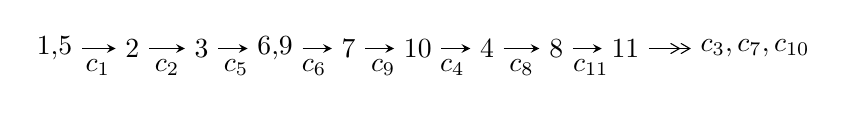
\begin{tikzpicture}[x=25pt, y=7pt]
	% node
	\node (A0) at (-1/8, 0) {1,5};
	\node (A1) at (1, 0) {2};
	\node (A2) at (2, 0) {3};
	\node (A3) at (49/16, 0) {6,9};
	\node (A4) at (33/8, 0) {7};
	\node (A5) at (41/8, 0) {10};
	\node (A6) at (49/8, 0) {4};
	\node (A7) at (57/8, 0) {8};
	\node (A8) at (65/8, 0) {11};
	\node (C1) at (1/2, -1) {$c_{1}$};
	\node (C2) at (3/2, -1) {$c_{2}$};
	\node (C3) at (5/2, -1) {$c_{5}$};
	\node (C4) at (29/8, -1) {$c_{6}$};
	\node (C5) at (37/8, -1) {$c_{9}$};
	\node (C6) at (45/8, -1) {$c_{4}$};
	\node (C7) at (53/8, -1) {$c_{8}$};
	\node (C8) at (61/8, -1) {$c_{11}$};
	\node (A9) at (10, 0) {$c_{3},c_{7},c_{10}$};

	% edge
	\draw[->,>=stealth]	
	(A0) edge (A1) (A1) edge (A2) (A2) edge (A3) (A3) edge (A4) (A4) edge (A5) (A5) edge (A6) (A6) edge (A7) (A7) edge (A8) ;
	\draw[->>,>={angle 60}]	
	(A8) edge (A9);
\end{tikzpicture} \\ 

\end{tabular} \\

\footnotetext{
The image of knot diagram is generated by the software ``\textbf{Draw programme}" developed by Andrew Bartholomew(\url{http://www.layer8.co.uk/maths/draw/index.htm\#Running-draw}), where we modified some parts for our purpose(\url{https://github.com/CATsTAILs/LinksPainter}).
}\phantom \\ \newline 
\centering \textbf{Ideals for irreducible components\footnotemark of $X_{\text{par}}$} 
 
\begin{align*}
I^u_{1}&=\langle 
2 u^8-6 u^7+u^6+3 u^5+15 u^4-13 u^3-10 u^2+b+3 u+3,\;u^8- u^7-5 u^6+3 u^5+7 u^4+7 u^3-15 u^2+2 a+2,\\
\phantom{I^u_{1}}&\phantom{= \langle  }u^9-5 u^8+7 u^7- u^6+5 u^5-21 u^4+11 u^3+8 u^2-2 u-2\rangle \\
I^u_{2}&=\langle 
- u^3- u^2+b+u+1,\;- u^4-2 u^3+u^2+2 a+u,\;u^5+2 u^4- u^3-3 u^2+2\rangle \\
I^u_{3}&=\langle 
- u^2 a- a u+u^2+b+u-1,\;u^2 a+a^2-5 u^2-3 a-2 u+11,\;u^3+u^2-2 u-1\rangle \\
\\
\end{align*}
\raggedright * 3 irreducible components of $\dim_{\mathbb{C}}=0$, with total 20 representations.\\
\footnotetext{All coefficients of polynomials are rational numbers. But the coefficients are sometimes approximated in decimal forms when there is not enough margin.}
\newpage
\renewcommand{\arraystretch}{1}
\centering \section*{I. $I^u_{1}= \langle 2 u^8-6 u^7+\cdots+b+3,\;u^8- u^7+\cdots+2 a+2,\;u^9-5 u^8+\cdots-2 u-2 \rangle$}
\flushleft \textbf{(i) Arc colorings}\\
\begin{tabular}{m{7pt} m{180pt} m{7pt} m{180pt} }
\flushright $a_{1}=$&$\begin{pmatrix}1\\0\end{pmatrix}$ \\
\flushright $a_{5}=$&$\begin{pmatrix}0\\u\end{pmatrix}$ \\
\flushright $a_{2}=$&$\begin{pmatrix}1\\u^2\end{pmatrix}$ \\
\flushright $a_{3}=$&$\begin{pmatrix}- u^2+1\\u^2\end{pmatrix}$ \\
\flushright $a_{6}=$&$\begin{pmatrix}- u\\- u^3+u\end{pmatrix}$ \\
\flushright $a_{9}=$&$\begin{pmatrix}-\frac{1}{2} u^8+\frac{1}{2} u^7+\cdots+\frac{15}{2} u^2-1\\-2 u^8+6 u^7- u^6-3 u^5-15 u^4+13 u^3+10 u^2-3 u-3\end{pmatrix}$ \\
\flushright $a_{7}=$&$\begin{pmatrix}-\frac{3}{2} u^8+\frac{11}{2} u^7+\cdots-3 u-2\\- u^8+4 u^7-3 u^6- u^5-8 u^4+12 u^3+u^2- u-1\end{pmatrix}$ \\
\flushright $a_{10}=$&$\begin{pmatrix}\frac{3}{2} u^8-\frac{11}{2} u^7+\cdots+3 u+2\\-2 u^8+6 u^7- u^6-3 u^5-15 u^4+13 u^3+10 u^2-3 u-3\end{pmatrix}$ \\
\flushright $a_{4}=$&$\begin{pmatrix}\frac{1}{2} u^8-\frac{3}{2} u^7+\cdots+u+1\\- u^8+3 u^7- u^6- u^5-7 u^4+7 u^3+4 u^2- u-1\end{pmatrix}$ \\
\flushright $a_{8}=$&$\begin{pmatrix}-\frac{1}{2} u^8+\frac{1}{2} u^7+\cdots+\frac{15}{2} u^2-1\\2 u^8-6 u^7+2 u^6+u^5+14 u^4-13 u^3-4 u^2+2 u+1\end{pmatrix}$ \\
\flushright $a_{11}=$&$\begin{pmatrix}\frac{3}{2} u^8-\frac{11}{2} u^7+\cdots+3 u+2\\u^8-5 u^7+5 u^6+2 u^5+8 u^4-18 u^3- u^2+4 u+1\end{pmatrix}$\\ \flushright $a_{11}=$&$\begin{pmatrix}\frac{3}{2} u^8-\frac{11}{2} u^7+\cdots+3 u+2\\u^8-5 u^7+5 u^6+2 u^5+8 u^4-18 u^3- u^2+4 u+1\end{pmatrix}$\\&\end{tabular}
\flushleft \textbf{(ii) Obstruction class $= -1$}\\~\\
\flushleft \textbf{(iii) Cusp Shapes $= -3 u^8+13 u^7-14 u^6+u^5-20 u^4+46 u^3-14 u^2-12 u-6$}\\~\\
\newpage\renewcommand{\arraystretch}{1}
\flushleft \textbf{(iv) u-Polynomials at the component}\newline \\
\begin{tabular}{m{50pt}|m{274pt}}
Crossings & \hspace{64pt}u-Polynomials at each crossing \\
\hline $$\begin{aligned}c_{1},c_{5}\end{aligned}$$&$\begin{aligned}
&u^9+5 u^8+7 u^7+u^6+5 u^5+21 u^4+11 u^3-8 u^2-2 u+2
\end{aligned}$\\
\hline $$\begin{aligned}c_{2}\end{aligned}$$&$\begin{aligned}
&u^9+11 u^8+\cdots+36 u+4
\end{aligned}$\\
\hline $$\begin{aligned}c_{3},c_{4},c_{10}\end{aligned}$$&$\begin{aligned}
&u^9+7 u^7+2 u^6+18 u^5+8 u^4+16 u^3+7 u^2+2 u+1
\end{aligned}$\\
\hline $$\begin{aligned}c_{6},c_{9}\end{aligned}$$&$\begin{aligned}
&u^9-2 u^8-3 u^7+8 u^6+6 u^5-10 u^4-10 u^3+3 u^2+8 u+1
\end{aligned}$\\
\hline $$\begin{aligned}c_{7}\end{aligned}$$&$\begin{aligned}
&u^9+6 u^8+19 u^7+38 u^6+54 u^5+56 u^4+49 u^3+36 u^2+16 u+2
\end{aligned}$\\
\hline $$\begin{aligned}c_{8}\end{aligned}$$&$\begin{aligned}
&u^9+u^8-8 u^7-4 u^6+21 u^5+3 u^4-3 u^3-5 u^2+u+1
\end{aligned}$\\
\hline $$\begin{aligned}c_{11}\end{aligned}$$&$\begin{aligned}
&u^9-8 u^8+30 u^7-69 u^6+106 u^5-109 u^4+69 u^3-18 u^2-8 u+8
\end{aligned}$\\
\hline
\end{tabular}\\~\\
\newpage\renewcommand{\arraystretch}{1}
\flushleft \textbf{(v) Riley Polynomials at the component}\newline \\
\begin{tabular}{m{50pt}|m{274pt}}
Crossings & \hspace{64pt}Riley Polynomials at each crossing \\
\hline $$\begin{aligned}c_{1},c_{5}\end{aligned}$$&$\begin{aligned}
&y^9-11 y^8+\cdots+36 y-4
\end{aligned}$\\
\hline $$\begin{aligned}c_{2}\end{aligned}$$&$\begin{aligned}
&y^9-23 y^8+\cdots-240 y-16
\end{aligned}$\\
\hline $$\begin{aligned}c_{3},c_{4},c_{10}\end{aligned}$$&$\begin{aligned}
&y^9+14 y^8+85 y^7+280 y^6+520 y^5+512 y^4+212 y^3- y^2-10 y-1
\end{aligned}$\\
\hline $$\begin{aligned}c_{6},c_{9}\end{aligned}$$&$\begin{aligned}
&y^9-10 y^8+\cdots+58 y-1
\end{aligned}$\\
\hline $$\begin{aligned}c_{7}\end{aligned}$$&$\begin{aligned}
&y^9+2 y^8+13 y^7+34 y^6+122 y^5+4 y^4-55 y^3+48 y^2+112 y-4
\end{aligned}$\\
\hline $$\begin{aligned}c_{8}\end{aligned}$$&$\begin{aligned}
&y^9-17 y^8+\cdots+11 y-1
\end{aligned}$\\
\hline $$\begin{aligned}c_{11}\end{aligned}$$&$\begin{aligned}
&y^9-4 y^8+8 y^7-7 y^6+30 y^5-89 y^4+245 y^3+316 y^2+352 y-64
\end{aligned}$\\
\hline
\end{tabular}\\~\\
\newpage\flushleft \textbf{(vi) Complex Volumes and Cusp Shapes}
$$\begin{array}{c|c|c}  
\text{Solutions to }I^u_{1}& \I (\text{vol} + \sqrt{-1}CS) & \text{Cusp shape}\\
 \hline 
\begin{aligned}
u &= -0.827217 + 1.065600 I \\
a &= \phantom{-}0.127211 + 0.403713 I \\
b &= \phantom{-}1.189760 - 0.208029 I\end{aligned}
 & \phantom{-}4.50943 + 3.60395 I & -7.94742 - 3.61538 I \\ \hline\begin{aligned}
u &= -0.827217 - 1.065600 I \\
a &= \phantom{-}0.127211 - 0.403713 I \\
b &= \phantom{-}1.189760 + 0.208029 I\end{aligned}
 & \phantom{-}4.50943 - 3.60395 I & -7.94742 + 3.61538 I \\ \hline\begin{aligned}
u &= \phantom{-}0.637971\phantom{ +0.000000I} \\
a &= \phantom{-}0.581775\phantom{ +0.000000I} \\
b &= -0.134369\phantom{ +0.000000I}\end{aligned}
 & -0.867730\phantom{ +0.000000I} & -11.0840\phantom{ +0.000000I} \\ \hline\begin{aligned}
u &= -0.390331 + 0.211849 I \\
a &= -0.15178 - 1.44152 I \\
b &= -0.619342 - 0.660345 I\end{aligned}
 & -0.58699 - 1.71933 I & -2.65828 + 4.51037 I \\ \hline\begin{aligned}
u &= -0.390331 - 0.211849 I \\
a &= -0.15178 + 1.44152 I \\
b &= -0.619342 + 0.660345 I\end{aligned}
 & -0.58699 + 1.71933 I & -2.65828 - 4.51037 I \\ \hline\begin{aligned}
u &= \phantom{-}1.60275 + 0.27471 I \\
a &= -1.057300 + 0.502009 I \\
b &= -1.245760 - 0.193497 I\end{aligned}
 & -7.17964 - 0.81901 I & -9.63369 + 0.38923 I \\ \hline\begin{aligned}
u &= \phantom{-}1.60275 - 0.27471 I \\
a &= -1.057300 - 0.502009 I \\
b &= -1.245760 + 0.193497 I\end{aligned}
 & -7.17964 + 0.81901 I & -9.63369 - 0.38923 I \\ \hline\begin{aligned}
u &= \phantom{-}1.79582 + 0.27938 I \\
a &= \phantom{-}1.290980 + 0.002356 I \\
b &= \phantom{-}1.74253 + 0.93792 I\end{aligned}
 & -4.53360 - 8.88256 I & -8.21864 + 4.17646 I \\ \hline\begin{aligned}
u &= \phantom{-}1.79582 - 0.27938 I \\
a &= \phantom{-}1.290980 - 0.002356 I \\
b &= \phantom{-}1.74253 - 0.93792 I\end{aligned}
 & -4.53360 + 8.88256 I & -8.21864 - 4.17646 I\\
 \hline 
 \end{array}$$\newpage\newpage\renewcommand{\arraystretch}{1}
\centering \section*{II. $I^u_{2}= \langle - u^3- u^2+b+u+1,\;- u^4-2 u^3+u^2+2 a+u,\;u^5+2 u^4- u^3-3 u^2+2 \rangle$}
\flushleft \textbf{(i) Arc colorings}\\
\begin{tabular}{m{7pt} m{180pt} m{7pt} m{180pt} }
\flushright $a_{1}=$&$\begin{pmatrix}1\\0\end{pmatrix}$ \\
\flushright $a_{5}=$&$\begin{pmatrix}0\\u\end{pmatrix}$ \\
\flushright $a_{2}=$&$\begin{pmatrix}1\\u^2\end{pmatrix}$ \\
\flushright $a_{3}=$&$\begin{pmatrix}- u^2+1\\u^2\end{pmatrix}$ \\
\flushright $a_{6}=$&$\begin{pmatrix}- u\\- u^3+u\end{pmatrix}$ \\
\flushright $a_{9}=$&$\begin{pmatrix}\frac{1}{2} u^4+u^3-\frac{1}{2} u^2-\frac{1}{2} u\\u^3+u^2- u-1\end{pmatrix}$ \\
\flushright $a_{7}=$&$\begin{pmatrix}-\frac{1}{2} u^4+\frac{3}{2} u^2-\frac{1}{2} u-1\\u^2+u-1\end{pmatrix}$ \\
\flushright $a_{10}=$&$\begin{pmatrix}\frac{1}{2} u^4-\frac{3}{2} u^2+\frac{1}{2} u+1\\u^3+u^2- u-1\end{pmatrix}$ \\
\flushright $a_{4}=$&$\begin{pmatrix}\frac{1}{2} u^4+u^3-\frac{3}{2} u^2-\frac{3}{2} u+2\\u^2+u-1\end{pmatrix}$ \\
\flushright $a_{8}=$&$\begin{pmatrix}\frac{1}{2} u^4+u^3-\frac{1}{2} u^2-\frac{1}{2} u\\u^2-1\end{pmatrix}$ \\
\flushright $a_{11}=$&$\begin{pmatrix}\frac{1}{2} u^4-\frac{3}{2} u^2+\frac{1}{2} u+1\\u^4+2 u^3- u^2-2 u+1\end{pmatrix}$\\ \flushright $a_{11}=$&$\begin{pmatrix}\frac{1}{2} u^4-\frac{3}{2} u^2+\frac{1}{2} u+1\\u^4+2 u^3- u^2-2 u+1\end{pmatrix}$\\&\end{tabular}
\flushleft \textbf{(ii) Obstruction class $= 1$}\\~\\
\flushleft \textbf{(iii) Cusp Shapes $= -2 u^4-2 u^3+u^2-2 u-10$}\\~\\
\newpage\renewcommand{\arraystretch}{1}
\flushleft \textbf{(iv) u-Polynomials at the component}\newline \\
\begin{tabular}{m{50pt}|m{274pt}}
Crossings & \hspace{64pt}u-Polynomials at each crossing \\
\hline $$\begin{aligned}c_{1}\end{aligned}$$&$\begin{aligned}
&u^5+2 u^4- u^3-3 u^2+2
\end{aligned}$\\
\hline $$\begin{aligned}c_{2}\end{aligned}$$&$\begin{aligned}
&u^5+6 u^4+13 u^3+17 u^2+12 u+4
\end{aligned}$\\
\hline $$\begin{aligned}c_{3},c_{10}\end{aligned}$$&$\begin{aligned}
&u^5+2 u^3+u^2-3 u+1
\end{aligned}$\\
\hline $$\begin{aligned}c_{4}\end{aligned}$$&$\begin{aligned}
&u^5+2 u^3- u^2-3 u-1
\end{aligned}$\\
\hline $$\begin{aligned}c_{5}\end{aligned}$$&$\begin{aligned}
&u^5-2 u^4- u^3+3 u^2-2
\end{aligned}$\\
\hline $$\begin{aligned}c_{6},c_{9}\end{aligned}$$&$\begin{aligned}
&u^5-2 u^4+u^2- u-1
\end{aligned}$\\
\hline $$\begin{aligned}c_{7}\end{aligned}$$&$\begin{aligned}
&u^5+3 u^4+2 u^3- u^2-2 u-2
\end{aligned}$\\
\hline $$\begin{aligned}c_{8}\end{aligned}$$&$\begin{aligned}
&u^5- u^4- u^3-4 u^2-2 u-1
\end{aligned}$\\
\hline $$\begin{aligned}c_{11}\end{aligned}$$&$\begin{aligned}
&u^5+u^4- u^3+2 u-1
\end{aligned}$\\
\hline
\end{tabular}\\~\\
\newpage\renewcommand{\arraystretch}{1}
\flushleft \textbf{(v) Riley Polynomials at the component}\newline \\
\begin{tabular}{m{50pt}|m{274pt}}
Crossings & \hspace{64pt}Riley Polynomials at each crossing \\
\hline $$\begin{aligned}c_{1},c_{5}\end{aligned}$$&$\begin{aligned}
&y^5-6 y^4+13 y^3-17 y^2+12 y-4
\end{aligned}$\\
\hline $$\begin{aligned}c_{2}\end{aligned}$$&$\begin{aligned}
&y^5-10 y^4-11 y^3-25 y^2+8 y-16
\end{aligned}$\\
\hline $$\begin{aligned}c_{3},c_{4},c_{10}\end{aligned}$$&$\begin{aligned}
&y^5+4 y^4-2 y^3-13 y^2+7 y-1
\end{aligned}$\\
\hline $$\begin{aligned}c_{6},c_{9}\end{aligned}$$&$\begin{aligned}
&y^5-4 y^4+2 y^3-5 y^2+3 y-1
\end{aligned}$\\
\hline $$\begin{aligned}c_{7}\end{aligned}$$&$\begin{aligned}
&y^5-5 y^4+6 y^3+3 y^2-4
\end{aligned}$\\
\hline $$\begin{aligned}c_{8}\end{aligned}$$&$\begin{aligned}
&y^5-3 y^4-11 y^3-14 y^2-4 y-1
\end{aligned}$\\
\hline $$\begin{aligned}c_{11}\end{aligned}$$&$\begin{aligned}
&y^5-3 y^4+5 y^3-2 y^2+4 y-1
\end{aligned}$\\
\hline
\end{tabular}\\~\\
\newpage\flushleft \textbf{(vi) Complex Volumes and Cusp Shapes}
$$\begin{array}{c|c|c}  
\text{Solutions to }I^u_{2}& \I (\text{vol} + \sqrt{-1}CS) & \text{Cusp shape}\\
 \hline 
\begin{aligned}
u &= \phantom{-}0.886428 + 0.266186 I \\
a &= -0.148382 + 0.576930 I \\
b &= -0.663438 + 0.814334 I\end{aligned}
 & -1.42879 + 1.52428 I & -12.65090 - 2.62716 I \\ \hline\begin{aligned}
u &= \phantom{-}0.886428 - 0.266186 I \\
a &= -0.148382 - 0.576930 I \\
b &= -0.663438 - 0.814334 I\end{aligned}
 & -1.42879 - 1.52428 I & -12.65090 + 2.62716 I \\ \hline\begin{aligned}
u &= -0.972160 + 0.575992 I \\
a &= -0.210793 + 1.027090 I \\
b &= \phantom{-}0.634295 - 0.253899 I\end{aligned}
 & \phantom{-}6.00798 + 2.19755 I & -5.78391 - 2.40841 I \\ \hline\begin{aligned}
u &= -0.972160 - 0.575992 I \\
a &= -0.210793 - 1.027090 I \\
b &= \phantom{-}0.634295 + 0.253899 I\end{aligned}
 & \phantom{-}6.00798 - 2.19755 I & -5.78391 + 2.40841 I \\ \hline\begin{aligned}
u &= -1.82854\phantom{ +0.000000I} \\
a &= -1.28165\phantom{ +0.000000I} \\
b &= -1.94171\phantom{ +0.000000I}\end{aligned}
 & -12.4482\phantom{ +0.000000I} & -13.1300\phantom{ +0.000000I}\\
 \hline 
 \end{array}$$\newpage\newpage\renewcommand{\arraystretch}{1}
\centering \section*{III. $I^u_{3}= \langle - u^2 a- a u+u^2+b+u-1,\;u^2 a+a^2-5 u^2-3 a-2 u+11,\;u^3+u^2-2 u-1 \rangle$}
\flushleft \textbf{(i) Arc colorings}\\
\begin{tabular}{m{7pt} m{180pt} m{7pt} m{180pt} }
\flushright $a_{1}=$&$\begin{pmatrix}1\\0\end{pmatrix}$ \\
\flushright $a_{5}=$&$\begin{pmatrix}0\\u\end{pmatrix}$ \\
\flushright $a_{2}=$&$\begin{pmatrix}1\\u^2\end{pmatrix}$ \\
\flushright $a_{3}=$&$\begin{pmatrix}- u^2+1\\u^2\end{pmatrix}$ \\
\flushright $a_{6}=$&$\begin{pmatrix}- u\\u^2- u-1\end{pmatrix}$ \\
\flushright $a_{9}=$&$\begin{pmatrix}a\\u^2 a+a u- u^2- u+1\end{pmatrix}$ \\
\flushright $a_{7}=$&$\begin{pmatrix}- u^2 a- a u+u^2+a+u-2\\1\end{pmatrix}$ \\
\flushright $a_{10}=$&$\begin{pmatrix}- u^2 a- a u+u^2+a+u-1\\u^2 a+a u- u^2- u+1\end{pmatrix}$ \\
\flushright $a_{4}=$&$\begin{pmatrix}- a u-3 u^2- a- u+7\\a u+u^2+u-1\end{pmatrix}$ \\
\flushright $a_{8}=$&$\begin{pmatrix}a\\a u- u^2- u+1\end{pmatrix}$ \\
\flushright $a_{11}=$&$\begin{pmatrix}- u^2 a- a u+u^2+a+u-1\\1\end{pmatrix}$\\ \flushright $a_{11}=$&$\begin{pmatrix}- u^2 a- a u+u^2+a+u-1\\1\end{pmatrix}$\\&\end{tabular}
\flushleft \textbf{(ii) Obstruction class $= -1$}\\~\\
\flushleft \textbf{(iii) Cusp Shapes $= -6$}\\~\\
\newpage\renewcommand{\arraystretch}{1}
\flushleft \textbf{(iv) u-Polynomials at the component}\newline \\
\begin{tabular}{m{50pt}|m{274pt}}
Crossings & \hspace{64pt}u-Polynomials at each crossing \\
\hline $$\begin{aligned}c_{1},c_{5},c_{7}\end{aligned}$$&$\begin{aligned}
&(u^3- u^2-2 u+1)^2
\end{aligned}$\\
\hline $$\begin{aligned}c_{2}\end{aligned}$$&$\begin{aligned}
&(u^3+5 u^2+6 u+1)^2
\end{aligned}$\\
\hline $$\begin{aligned}c_{3},c_{4},c_{10}\end{aligned}$$&$\begin{aligned}
&u^6- u^5+2 u^4-4 u^3-2 u^2-8 u-1
\end{aligned}$\\
\hline $$\begin{aligned}c_{6},c_{9}\end{aligned}$$&$\begin{aligned}
&u^6- u^5-2 u^4+8 u^3-14 u^2+14 u-7
\end{aligned}$\\
\hline $$\begin{aligned}c_{8}\end{aligned}$$&$\begin{aligned}
&u^6+u^5-4 u^4-2 u^2-12 u-13
\end{aligned}$\\
\hline $$\begin{aligned}c_{11}\end{aligned}$$&$\begin{aligned}
&(u+1)^6
\end{aligned}$\\
\hline
\end{tabular}\\~\\
\newpage\renewcommand{\arraystretch}{1}
\flushleft \textbf{(v) Riley Polynomials at the component}\newline \\
\begin{tabular}{m{50pt}|m{274pt}}
Crossings & \hspace{64pt}Riley Polynomials at each crossing \\
\hline $$\begin{aligned}c_{1},c_{5},c_{7}\end{aligned}$$&$\begin{aligned}
&(y^3-5 y^2+6 y-1)^2
\end{aligned}$\\
\hline $$\begin{aligned}c_{2}\end{aligned}$$&$\begin{aligned}
&(y^3-13 y^2+26 y-1)^2
\end{aligned}$\\
\hline $$\begin{aligned}c_{3},c_{4},c_{10}\end{aligned}$$&$\begin{aligned}
&y^6+3 y^5-8 y^4-42 y^3-64 y^2-60 y+1
\end{aligned}$\\
\hline $$\begin{aligned}c_{6},c_{9}\end{aligned}$$&$\begin{aligned}
&y^6-5 y^5-8 y^4+6 y^3+49
\end{aligned}$\\
\hline $$\begin{aligned}c_{8}\end{aligned}$$&$\begin{aligned}
&y^6-9 y^5+12 y^4+14 y^3+108 y^2-92 y+169
\end{aligned}$\\
\hline $$\begin{aligned}c_{11}\end{aligned}$$&$\begin{aligned}
&(y-1)^6
\end{aligned}$\\
\hline
\end{tabular}\\~\\
\newpage\flushleft \textbf{(vi) Complex Volumes and Cusp Shapes}
$$\begin{array}{c|c|c}  
\text{Solutions to }I^u_{3}& \I (\text{vol} + \sqrt{-1}CS) & \text{Cusp shape}\\
 \hline 
\begin{aligned}
u &= \phantom{-}1.24698\phantom{ +0.000000I} \\
a &= \phantom{-}0.722521 + 0.457399 I \\
b &= \phantom{-}0.222521 + 1.281600 I\end{aligned}
 & \phantom{-}0.234991\phantom{ +0.000000I} & -6.00000\phantom{ +0.000000I} \\ \hline\begin{aligned}
u &= \phantom{-}1.24698\phantom{ +0.000000I} \\
a &= \phantom{-}0.722521 - 0.457399 I \\
b &= \phantom{-}0.222521 - 1.281600 I\end{aligned}
 & \phantom{-}0.234991\phantom{ +0.000000I} & -6.00000\phantom{ +0.000000I} \\ \hline\begin{aligned}
u &= -0.445042\phantom{ +0.000000I} \\
a &= \phantom{-}1.40097 + 2.98949 I \\
b &= \phantom{-}0.900969 - 0.738343 I\end{aligned}
 & \phantom{-}5.87476\phantom{ +0.000000I} & -6.00000\phantom{ +0.000000I} \\ \hline\begin{aligned}
u &= -0.445042\phantom{ +0.000000I} \\
a &= \phantom{-}1.40097 - 2.98949 I \\
b &= \phantom{-}0.900969 + 0.738343 I\end{aligned}
 & \phantom{-}5.87476\phantom{ +0.000000I} & -6.00000\phantom{ +0.000000I} \\ \hline\begin{aligned}
u &= -1.80194\phantom{ +0.000000I} \\
a &= \phantom{-}1.15958\phantom{ +0.000000I} \\
b &= \phantom{-}1.23060\phantom{ +0.000000I}\end{aligned}
 & -11.0446\phantom{ +0.000000I} & -6.00000\phantom{ +0.000000I} \\ \hline\begin{aligned}
u &= -1.80194\phantom{ +0.000000I} \\
a &= -1.40656\phantom{ +0.000000I} \\
b &= -2.47758\phantom{ +0.000000I}\end{aligned}
 & -11.0446\phantom{ +0.000000I} & -6.00000\phantom{ +0.000000I}\\
 \hline 
 \end{array}$$\newpage
\newpage\renewcommand{\arraystretch}{1}
\centering \section*{ IV. u-Polynomials}
\begin{tabular}{m{50pt}|m{274pt}}
Crossings & \hspace{64pt}u-Polynomials at each crossing \\
\hline $$\begin{aligned}c_{1}\end{aligned}$$&$\begin{aligned}
&(u^3- u^2-2 u+1)^2(u^5+2 u^4- u^3-3 u^2+2)\\
&\cdot(u^9+5 u^8+7 u^7+u^6+5 u^5+21 u^4+11 u^3-8 u^2-2 u+2)
\end{aligned}$\\
\hline $$\begin{aligned}c_{2}\end{aligned}$$&$\begin{aligned}
&(u^3+5 u^2+6 u+1)^2(u^5+6 u^4+13 u^3+17 u^2+12 u+4)\\
&\cdot(u^9+11 u^8+\cdots+36 u+4)
\end{aligned}$\\
\hline $$\begin{aligned}c_{3},c_{10}\end{aligned}$$&$\begin{aligned}
&(u^5+2 u^3+u^2-3 u+1)(u^6- u^5+2 u^4-4 u^3-2 u^2-8 u-1)\\
&\cdot(u^9+7 u^7+2 u^6+18 u^5+8 u^4+16 u^3+7 u^2+2 u+1)
\end{aligned}$\\
\hline $$\begin{aligned}c_{4}\end{aligned}$$&$\begin{aligned}
&(u^5+2 u^3- u^2-3 u-1)(u^6- u^5+2 u^4-4 u^3-2 u^2-8 u-1)\\
&\cdot(u^9+7 u^7+2 u^6+18 u^5+8 u^4+16 u^3+7 u^2+2 u+1)
\end{aligned}$\\
\hline $$\begin{aligned}c_{5}\end{aligned}$$&$\begin{aligned}
&(u^3- u^2-2 u+1)^2(u^5-2 u^4- u^3+3 u^2-2)\\
&\cdot(u^9+5 u^8+7 u^7+u^6+5 u^5+21 u^4+11 u^3-8 u^2-2 u+2)
\end{aligned}$\\
\hline $$\begin{aligned}c_{6},c_{9}\end{aligned}$$&$\begin{aligned}
&(u^5-2 u^4+u^2- u-1)(u^6- u^5-2 u^4+8 u^3-14 u^2+14 u-7)\\
&\cdot(u^9-2 u^8-3 u^7+8 u^6+6 u^5-10 u^4-10 u^3+3 u^2+8 u+1)
\end{aligned}$\\
\hline $$\begin{aligned}c_{7}\end{aligned}$$&$\begin{aligned}
&(u^3- u^2-2 u+1)^2(u^5+3 u^4+2 u^3- u^2-2 u-2)\\
&\cdot(u^9+6 u^8+19 u^7+38 u^6+54 u^5+56 u^4+49 u^3+36 u^2+16 u+2)
\end{aligned}$\\
\hline $$\begin{aligned}c_{8}\end{aligned}$$&$\begin{aligned}
&(u^5- u^4- u^3-4 u^2-2 u-1)(u^6+u^5-4 u^4-2 u^2-12 u-13)\\
&\cdot(u^9+u^8-8 u^7-4 u^6+21 u^5+3 u^4-3 u^3-5 u^2+u+1)
\end{aligned}$\\
\hline $$\begin{aligned}c_{11}\end{aligned}$$&$\begin{aligned}
&(u+1)^6(u^5+u^4- u^3+2 u-1)\\
&\cdot(u^9-8 u^8+30 u^7-69 u^6+106 u^5-109 u^4+69 u^3-18 u^2-8 u+8)
\end{aligned}$\\
\hline
\end{tabular}\newpage\renewcommand{\arraystretch}{1}
\centering \section*{ V. Riley Polynomials}
\begin{tabular}{m{50pt}|m{274pt}}
Crossings & \hspace{64pt}Riley Polynomials at each crossing \\
\hline $$\begin{aligned}c_{1},c_{5}\end{aligned}$$&$\begin{aligned}
&(y^3-5 y^2+6 y-1)^2(y^5-6 y^4+13 y^3-17 y^2+12 y-4)\\
&\cdot(y^9-11 y^8+\cdots+36 y-4)
\end{aligned}$\\
\hline $$\begin{aligned}c_{2}\end{aligned}$$&$\begin{aligned}
&(y^3-13 y^2+26 y-1)^2(y^5-10 y^4-11 y^3-25 y^2+8 y-16)\\
&\cdot(y^9-23 y^8+\cdots-240 y-16)
\end{aligned}$\\
\hline $$\begin{aligned}c_{3},c_{4},c_{10}\end{aligned}$$&$\begin{aligned}
&(y^5+4 y^4-2 y^3-13 y^2+7 y-1)\\
&\cdot(y^6+3 y^5-8 y^4-42 y^3-64 y^2-60 y+1)\\
&\cdot(y^9+14 y^8+85 y^7+280 y^6+520 y^5+512 y^4+212 y^3- y^2-10 y-1)
\end{aligned}$\\
\hline $$\begin{aligned}c_{6},c_{9}\end{aligned}$$&$\begin{aligned}
&(y^5-4 y^4+2 y^3-5 y^2+3 y-1)(y^6-5 y^5-8 y^4+6 y^3+49)\\
&\cdot(y^9-10 y^8+\cdots+58 y-1)
\end{aligned}$\\
\hline $$\begin{aligned}c_{7}\end{aligned}$$&$\begin{aligned}
&(y^3-5 y^2+6 y-1)^2(y^5-5 y^4+6 y^3+3 y^2-4)\\
&\cdot(y^9+2 y^8+13 y^7+34 y^6+122 y^5+4 y^4-55 y^3+48 y^2+112 y-4)
\end{aligned}$\\
\hline $$\begin{aligned}c_{8}\end{aligned}$$&$\begin{aligned}
&(y^5-3 y^4-11 y^3-14 y^2-4 y-1)\\
&\cdot(y^6-9 y^5+12 y^4+14 y^3+108 y^2-92 y+169)\\
&\cdot(y^9-17 y^8+\cdots+11 y-1)
\end{aligned}$\\
\hline $$\begin{aligned}c_{11}\end{aligned}$$&$\begin{aligned}
&(y-1)^6(y^5-3 y^4+5 y^3-2 y^2+4 y-1)\\
&\cdot(y^9-4 y^8+8 y^7-7 y^6+30 y^5-89 y^4+245 y^3+316 y^2+352 y-64)
\end{aligned}$\\
\hline
\end{tabular}
\vskip 2pc
\end{document}